\section{MLP}\label{sec:mlpbaseline}
In this section, we will introduce the first model, which we will refer to as the
baseline model, based on a Multi-Layer Perceptron.
We will analyze its architecture and the training phase.

%In questa sezione andremo ad introdurre il primo modello a cui faremo
%riferiento come baseline model, basato su MultiLayer Perceptron.
%Analizzeremo la sua architettura, la 
%fase di training e le sue performance finali.

\subsection{Architecture}
This neural network is designed to predict the instantaneous energy output over
a period of exactly 2 days.
To do this, it requires input data that includes the performance of the system
(features selected during the Preprocessing phase, see Chapter \ref{chap:datapreprocessing}) for exactly one day
before and one day after the period in question.
This enables it to understand how the system is performing and,
consequently, provide the energy output trend.
The model consists of 6 main layers:

%Questa rete neurale è progettata per prevedere l'andamento dell'energia istantanea prodotta durante un periodo di un buco di esattamente 2 giorni.
%Per farlo ha bisogno di avere come input l'andamento dell'impianto (features selezionate nella fase di preprocessing) di esattamente un giorno prima del
%buco e di un giorno dopo. In questo modo può riuscire a comprendere come l'impianto sta performando e quindi restituire l'andamento dell'energia.
%Il modello è formato da 6 livelli principali:

\begin{itemize}
	\item \textbf{Input layer}: This is the first layer of the network.
	      It takes two input tensors: \textit{before} and \textit{after}., representing the day before and the day after the specific period we want to
	      predict. They have the shape \verb|[BATCH_SIZE, 96, 33]|, where 96 is the number
	      of timestamps in our dataset that make up one day, and 33 represents the
	      features obtained from the Data Preprocessing phase.
	      These tensors are then flattened and concatenated to be passed to the subsequent layer.
	      The output of this layer goes through a Batch Normalization\cite{batchnorm} layer, and the
	      Rectified Linear Unit (ReLU)\cite{functions} activation function is used.

	      % è il primo livello della rete, prende in input 2 tensori: \textit{before} e \textit{after}. Questi stanno ad indicare rispettivamente il giorno prima e quello dopo del buco che vogliamo chiudere. Avranno la forma \verb|[BATCH_SIZE, 96, 33]|, dove \verb|96| è il numero di timestamp del nostro dataset che formano un giorno e \verb|33| sono le feature ottenute dalla fase di preprocessing dei dati. A questi verrà poi applicata un'operazione di Flatten ed infine concatenati per poter essere poi passati al layer successio.
	      %L'output di questo layer passa per un livello di Batch Normalization e viene utilizzata la ReLu come funzione di attivazione. 

	\item \textbf{Hidden layers}: In total, there are 3 layers, each of which takes the
	      output of the previous layer as input and reduces the number of neurons by approximately half. The 3 hidden layers are composed of 3069, 1527, and 986 nodes, respectively.
	      Batch Normalization\cite{batchnorm} is applied to the result, and the Rectified Linear Unit (ReLU)\cite{functions}
	      is used as the activation function.
	      %{\bf (*VP* aggiungerei in maniera esplicita il numero dei nodi degli hidden layer)}
	      %in totale 4, ognuno prende in input il risultato del layer precedente e va a dimezzare il numero dei neuroni. Al risultato viene applicata un'operazione di Batch Normalization e utilizzata la ReLu come funzione di attivazione.

	\item \textbf{Output layer}: The final layer of our network, it takes the result from the
	      previous layer and outputs the value of the Instantaneous Energy Produced
	      during the specific period.
	      It produces a tensor with a shape of \verb|[BATCH_SIZE, 192, 1]|.
	      The SoftPlus\cite{functions} function is used as the final activation function.

	      %ultimo layer della nostra rete, dal risultato del layer precedente riporta come output il valore dell'Energia Istantanea Prodotta durante il buco, un tensore di forma \verb|[BATCH_SIZE, 192, 1]|. Viene utilizzata la SoftPlus come funzione di attivazione finale.
\end{itemize}

\begin{figure}[H]
	\centering
	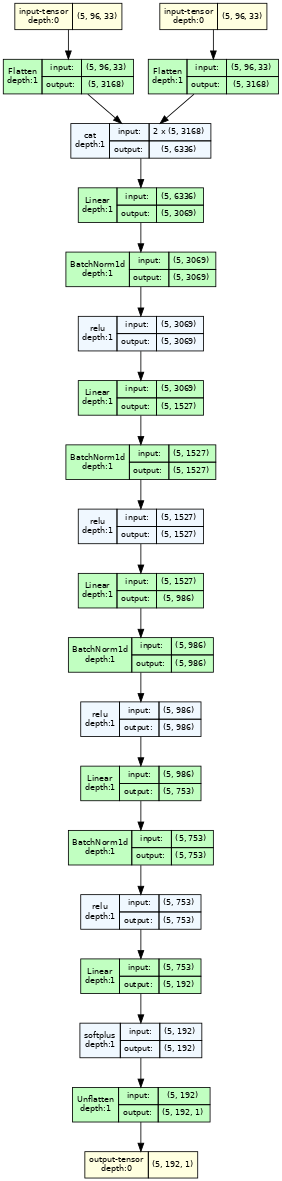
\includegraphics[height=.9\textheight]{chapters/3_models/imgs/ufcnmodel.png}
	\caption{Beseline Model architecture visualization.}\label{fig:baselinemodelarch}
\end{figure}

\subsection{Training}
The model was trained by artificially creating gaps of two days in length within the
training dataset.
These gaps were passed to the network in the format described earlier,
and the output result was compared to the actual instantaneous energy produced during the gap.
An \textit{Early Stopping}\cite{es} procedure was used
%\textbf{(*VP* a meno che tu non abbia implementato una procedura personalizzata, cambierei implemented in used)} 
to prevent training from continuing if
the model was not improving its performance.
A procedure, called \textit{Save Best}, has also been integrated,
which saves the model to a file whenever the Validation Loss improves.
The validation dataset was applied in this phase to assess the learning progress at the end
of each epoch.
A normalization procedure was applied to the model's output in relation to
that of the gap to ensure that the output starts exactly from the last value of the
instantaneous energy produced \textit{before} and ends exactly with the first value
of the energy produced \textit{after}.
{\bf (*VP* Non ho capito cosa fa e perchè usi questa normalizzazione)}
Adam\cite{adam} was used as the optimizer,
and L1Loss\cite{loss} (Equation~\ref{eq:l1loss}) served as the loss function. %{\bf (*VP*) non è la 3.2?}
We chose to set the batch size parameter to 10, the learning rate $\lambda$ to 0.01,
a maximum of 100 epochs, and a patience value of 20 for Early Stopping.

	{\bf (*VP* SE FAI IN TEMPO, CONSIDERA CHE TUTTE LE FIGURE DOVREBBERO ESSERE REFERENZIATE E SPIEGATE NEL TESTO. Le fig 3.2 e 3.3 le citi dove parli delle activation functions. La tab 3.1 la introduci dicendo una cosa tipo "In sintesi, in Tab 3.1 possiamo vedere il numerod i parametri totali etc...). Devi illustrare la fif 3.4 e soprattutto i grafici in 3.5. La speigazione di questi è essenziale perchè costituiscono a tutti gli effetti delle misure per comprendere quanto è costoso il training. Devi introdurre con una frase tipo "Per valutare il costo della procedura di training abbiamo utilizzato diverse misure, le elenchi e le spieghi rapidamente in un elenco puntato. Poi ti togli d'impiccio dicendo che per ognuna il corrispondente grafico in funzione del tempo di training è illustrato in Fig.3.5}

%Il modello è stato allenato creando, in modo artificiale, buchi di lunghezza
%pari a due giorni all'interno del dataset di training, passati alla rete nel formato
%descritto precedentemente e confrontato il risultato in output con l'effettiva energia istantanea
%prodotta del buco. \'{E} stata implementata una procedura di \textit{Early Stopping} per evitare
%di continuare l'allenamento anche se il modello non sta migliorando le sue performance. 
%\'{E} stata anche integrata una procedura, chiamata \textit{Save Best},
%che salva il modello su file ogni qualvolta la validation loss migliori.
%Il dataset di validation è stato applicato in questa fase per verificare lo stato di
%apprendimento alla fine di ogni epoca. All'output del modello è stata applicata una 
%procedura di normalizzazione dell'area rispetto a quella del buco per far si che la predizione
%parta esattamente dall'ultimo valore dell' energia istantanea prodotta di \textit{before} e
%termini esattamente con il primo valore di \textit{after}.
%\'{E} stato impiegato Adam come ottimizzatore e la L1Loss (Equation \ref{eq:l1loss}) come loss function.
%Abbiamo scelto di impostare il parametro batch size a 10, learning rate $\lambda$ a 0.01, 100
%come numero massimo di epoche e 20 come patience per l'Early Stopping.

\begin{gather}
	L = \{l_1,\dots,l_N\}^\top, \quad
	l_n = \left| x_n - y_n \right|,\\
	\ell(x,y) = \operatorname{mean}(L) \label{eq:l1loss}
\end{gather}

\begin{table}[H]
	\begin{center}
		\begin{tabular}[c]{l|l}

			\textbf{Total Parameters (\#)}     & 26543400 \\
			\textbf{Trainable Parameters (\#)} & 26543400 \\
			\textbf{Training Duration (s)}     & 24.0     \\
			\textbf{Model Size (MB)}           & 101.3
		\end{tabular}
	\end{center}
	\caption{Baseline Model specification.}\label{tab:ufcnspecs}
\end{table}

\begin{minipage}[t]{0.45\textwidth}
	\begin{figure}[H]
		\centering
		\begin{tikzpicture}
			\draw[->] (-3,0) -- (3,0) node[right] {$x$};
			\draw[->] (0,-1) -- (0,2) node[above] {$y$};
			\draw[dotted] (-3,-1) grid (3,2);
			\draw[color=blue, domain=-3:0] plot[id=logistic] function{0};
			\draw[color=blue, domain=0:2] plot[id=logistic] function{x};
		\end{tikzpicture}
		\caption{Rectified Linear Unit function. $ReLu(x) = \max(0, x)$}
		\label{fig:relu}
	\end{figure}
\end{minipage}%
\hspace{.5cm}
\begin{minipage}[t]{0.45\textwidth}
	\begin{figure}[H]
		\centering
		\begin{tikzpicture}
			\draw[->] (-3,0) -- (3,0) node[right] {$x$};
			\draw[->] (0,-1) -- (0,2) node[above] {$y$};
			\draw[dotted] (-3,-1) grid (3,2);
			\draw[color=blue, domain=-3:2] plot[id=logistic] function{log(1+exp(x))};
		\end{tikzpicture}
		\caption{SoftPlus function. $SoftPlus(x) = \frac{1}{\beta} \log(1+e^{\beta x})$}
		\label{fig:softplus}
	\end{figure}
\end{minipage}

\begin{figure}[H]
	\centering
	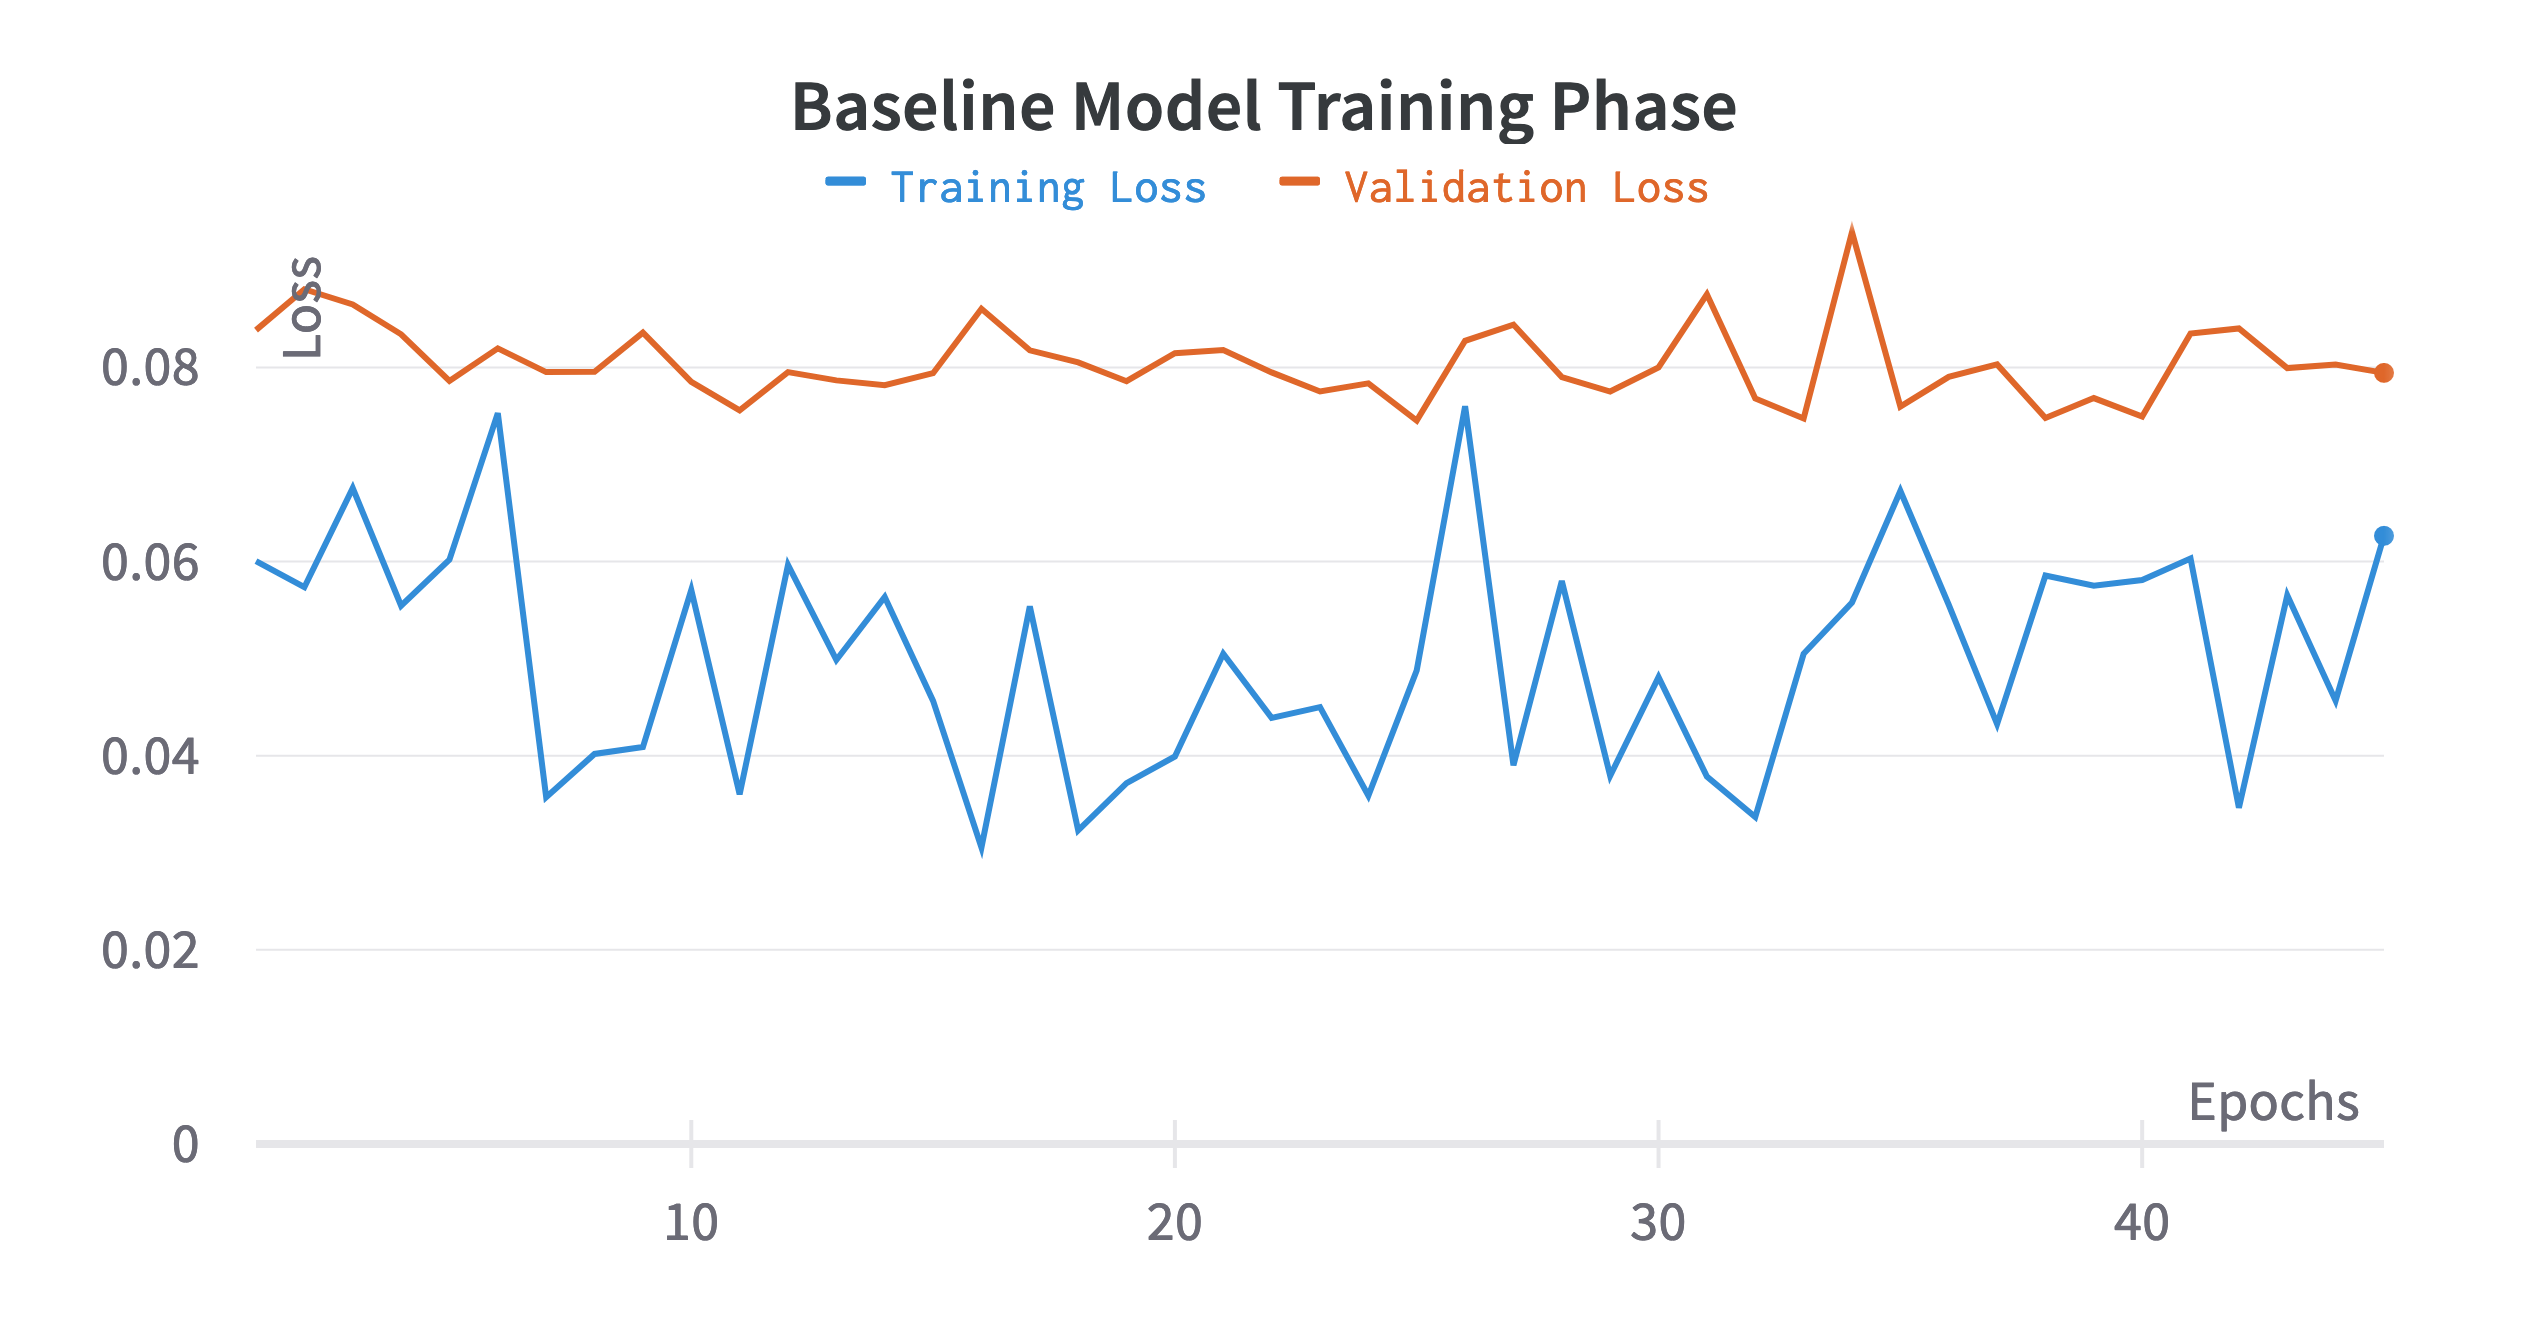
\includegraphics[width=.8\textwidth]{chapters/3_models/imgs/ufnc/ufnctraining.png}
	\caption{The chart displays the loss progression during the training phase. The blue line represents the Training Loss, while the orange line represents the Validation Loss.}
	\label{fig:ufcntraining}
\end{figure}

\begin{figure}[H]
	\centering
	\begin{subfigure}{0.43\textwidth}
		\centering
		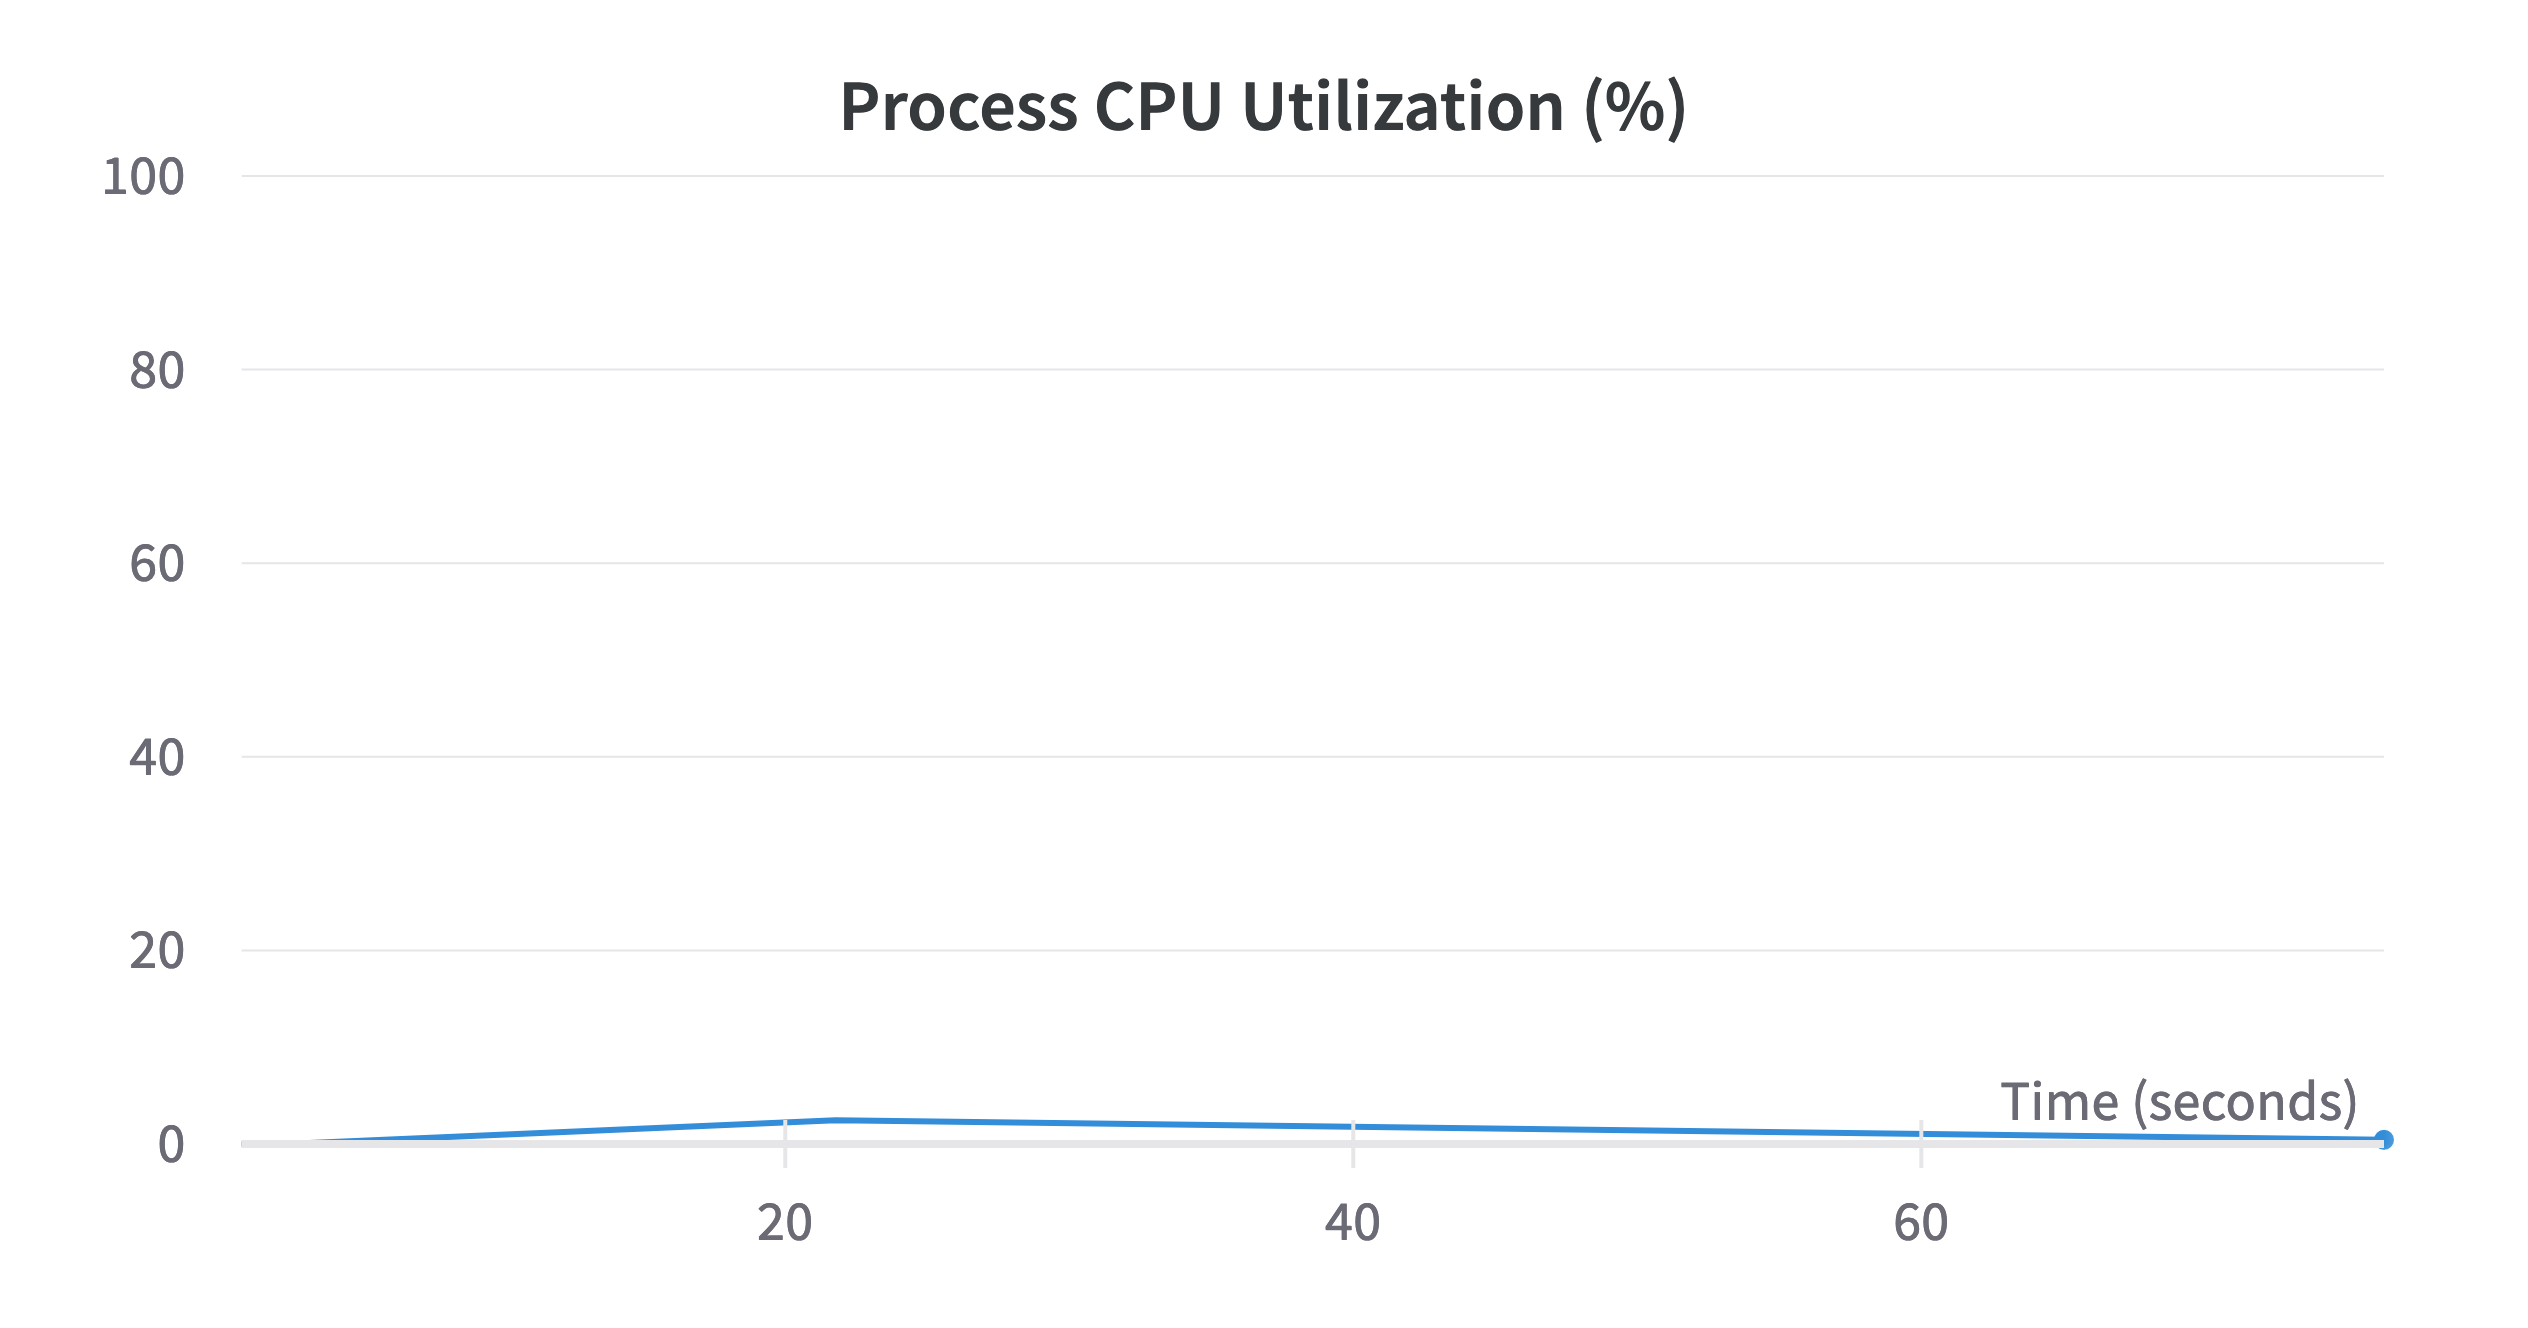
\includegraphics[width=\textwidth]{chapters/3_models/imgs/ufnc/ufcncpusage.png}
	\end{subfigure}
	\hspace{.5cm}
	\begin{subfigure}{0.43\textwidth}
		\centering
		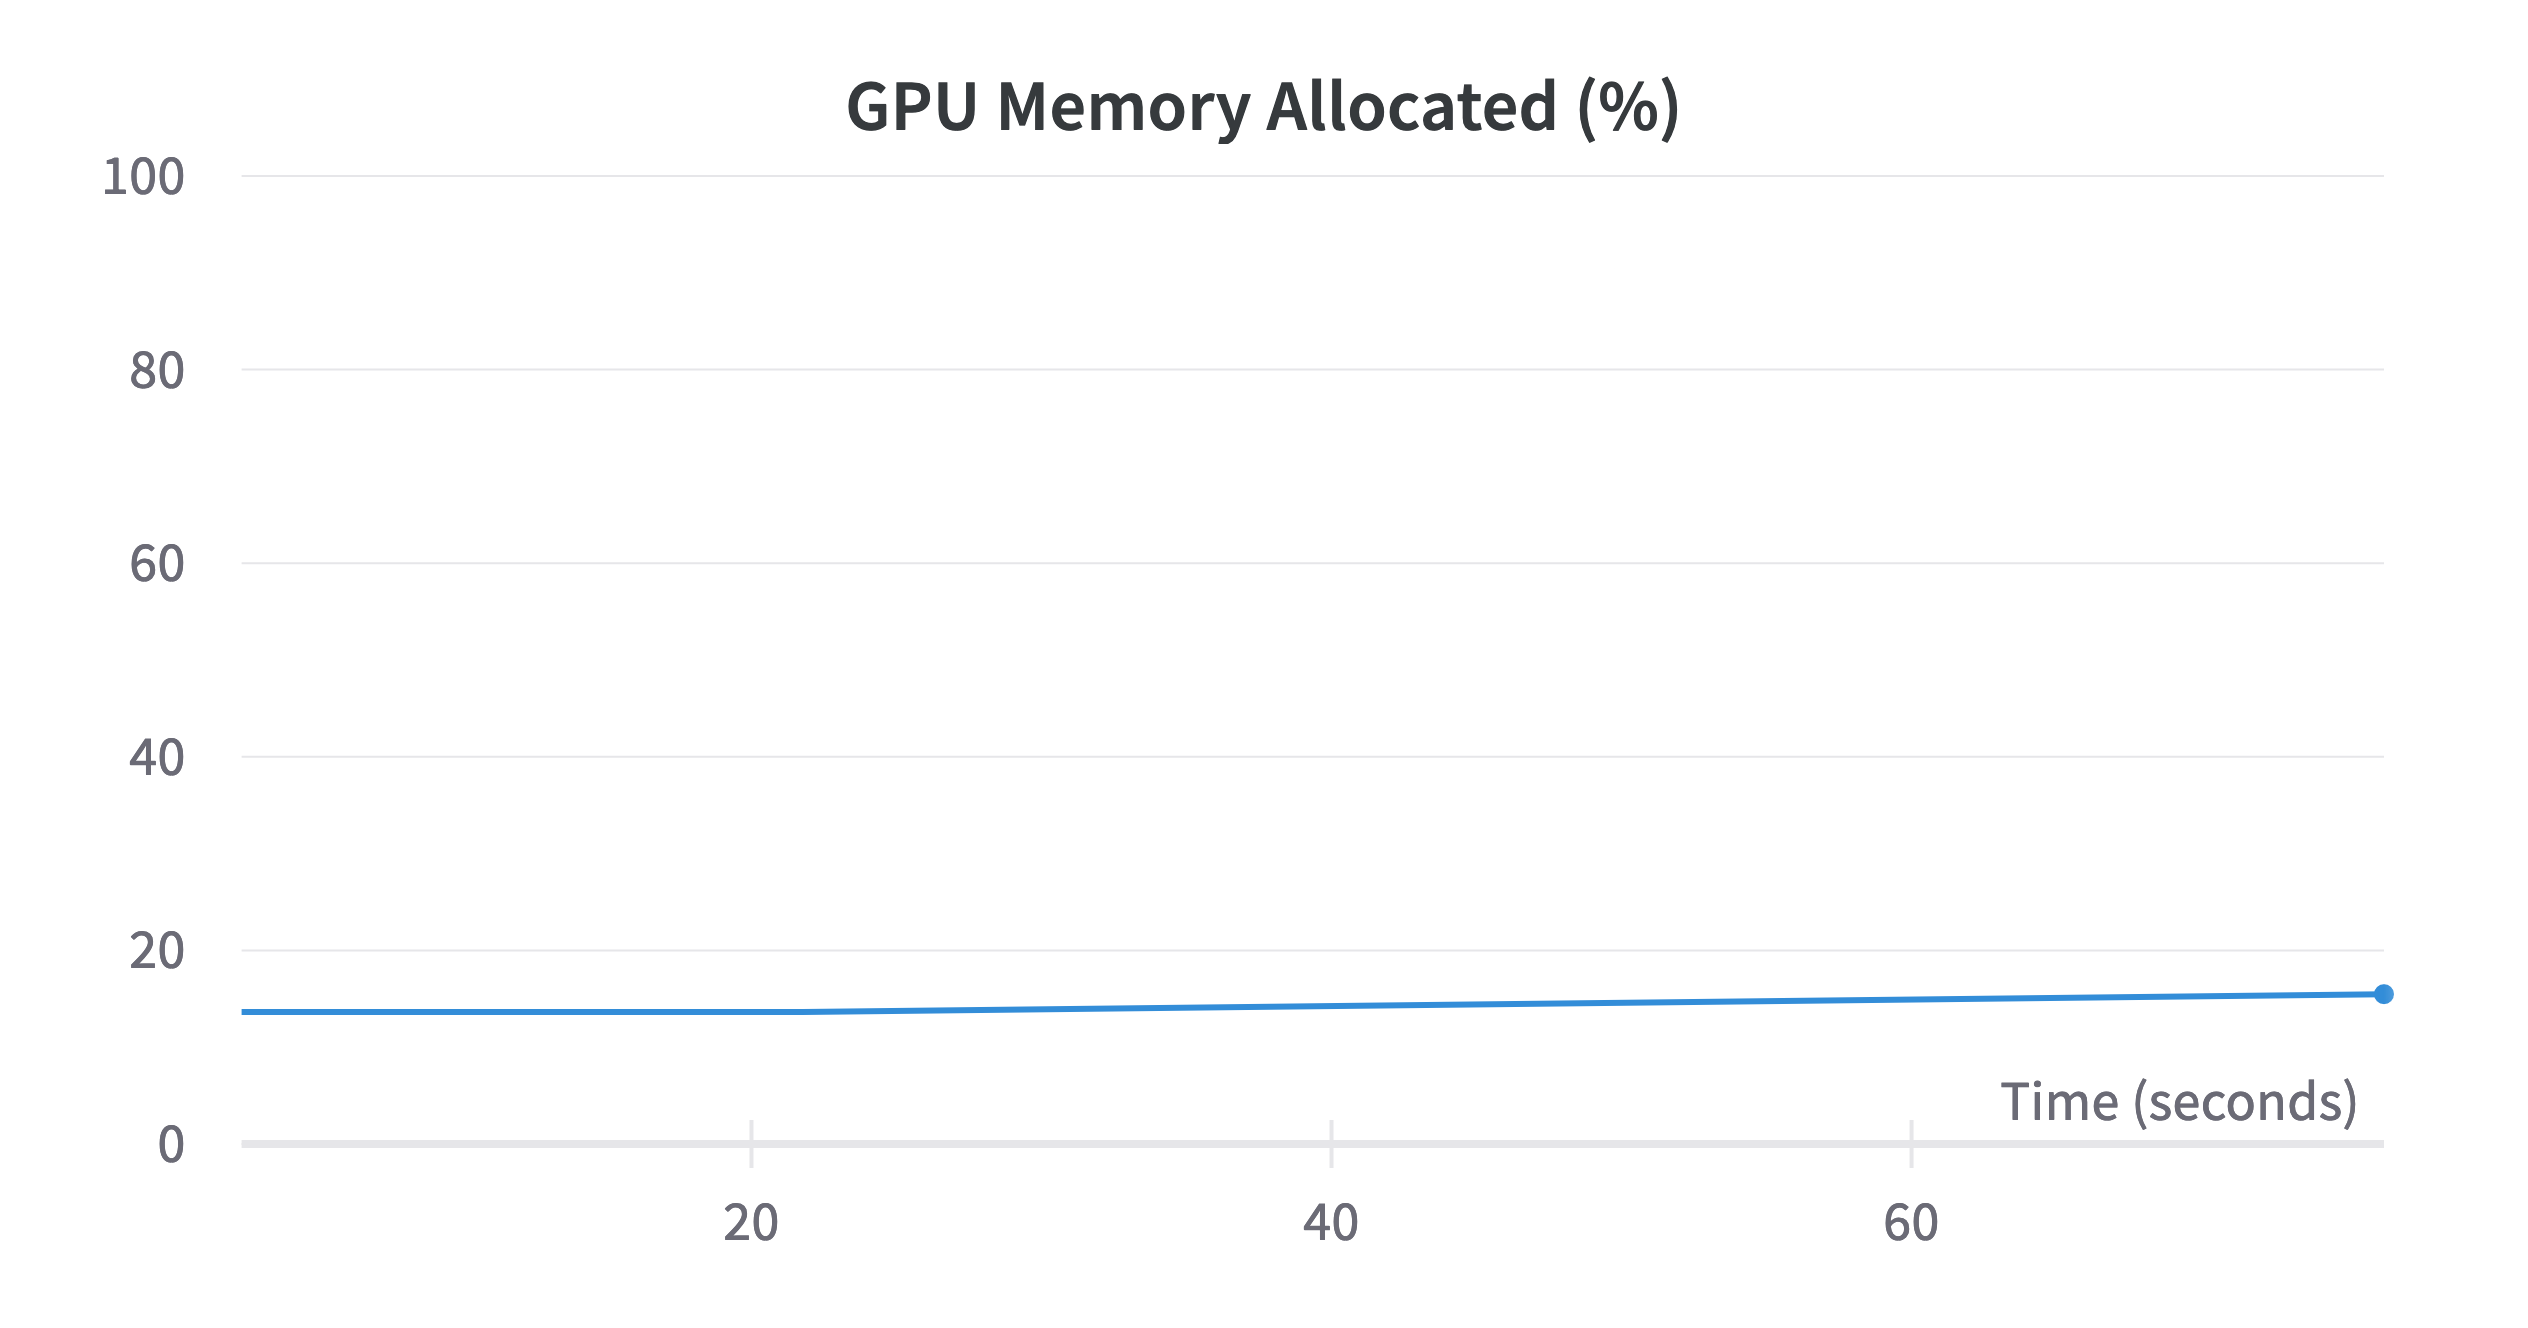
\includegraphics[width=\textwidth]{chapters/3_models/imgs/ufnc/ufcnmem.png}
	\end{subfigure}\\
	\begin{subfigure}{0.43\textwidth}
		\centering
		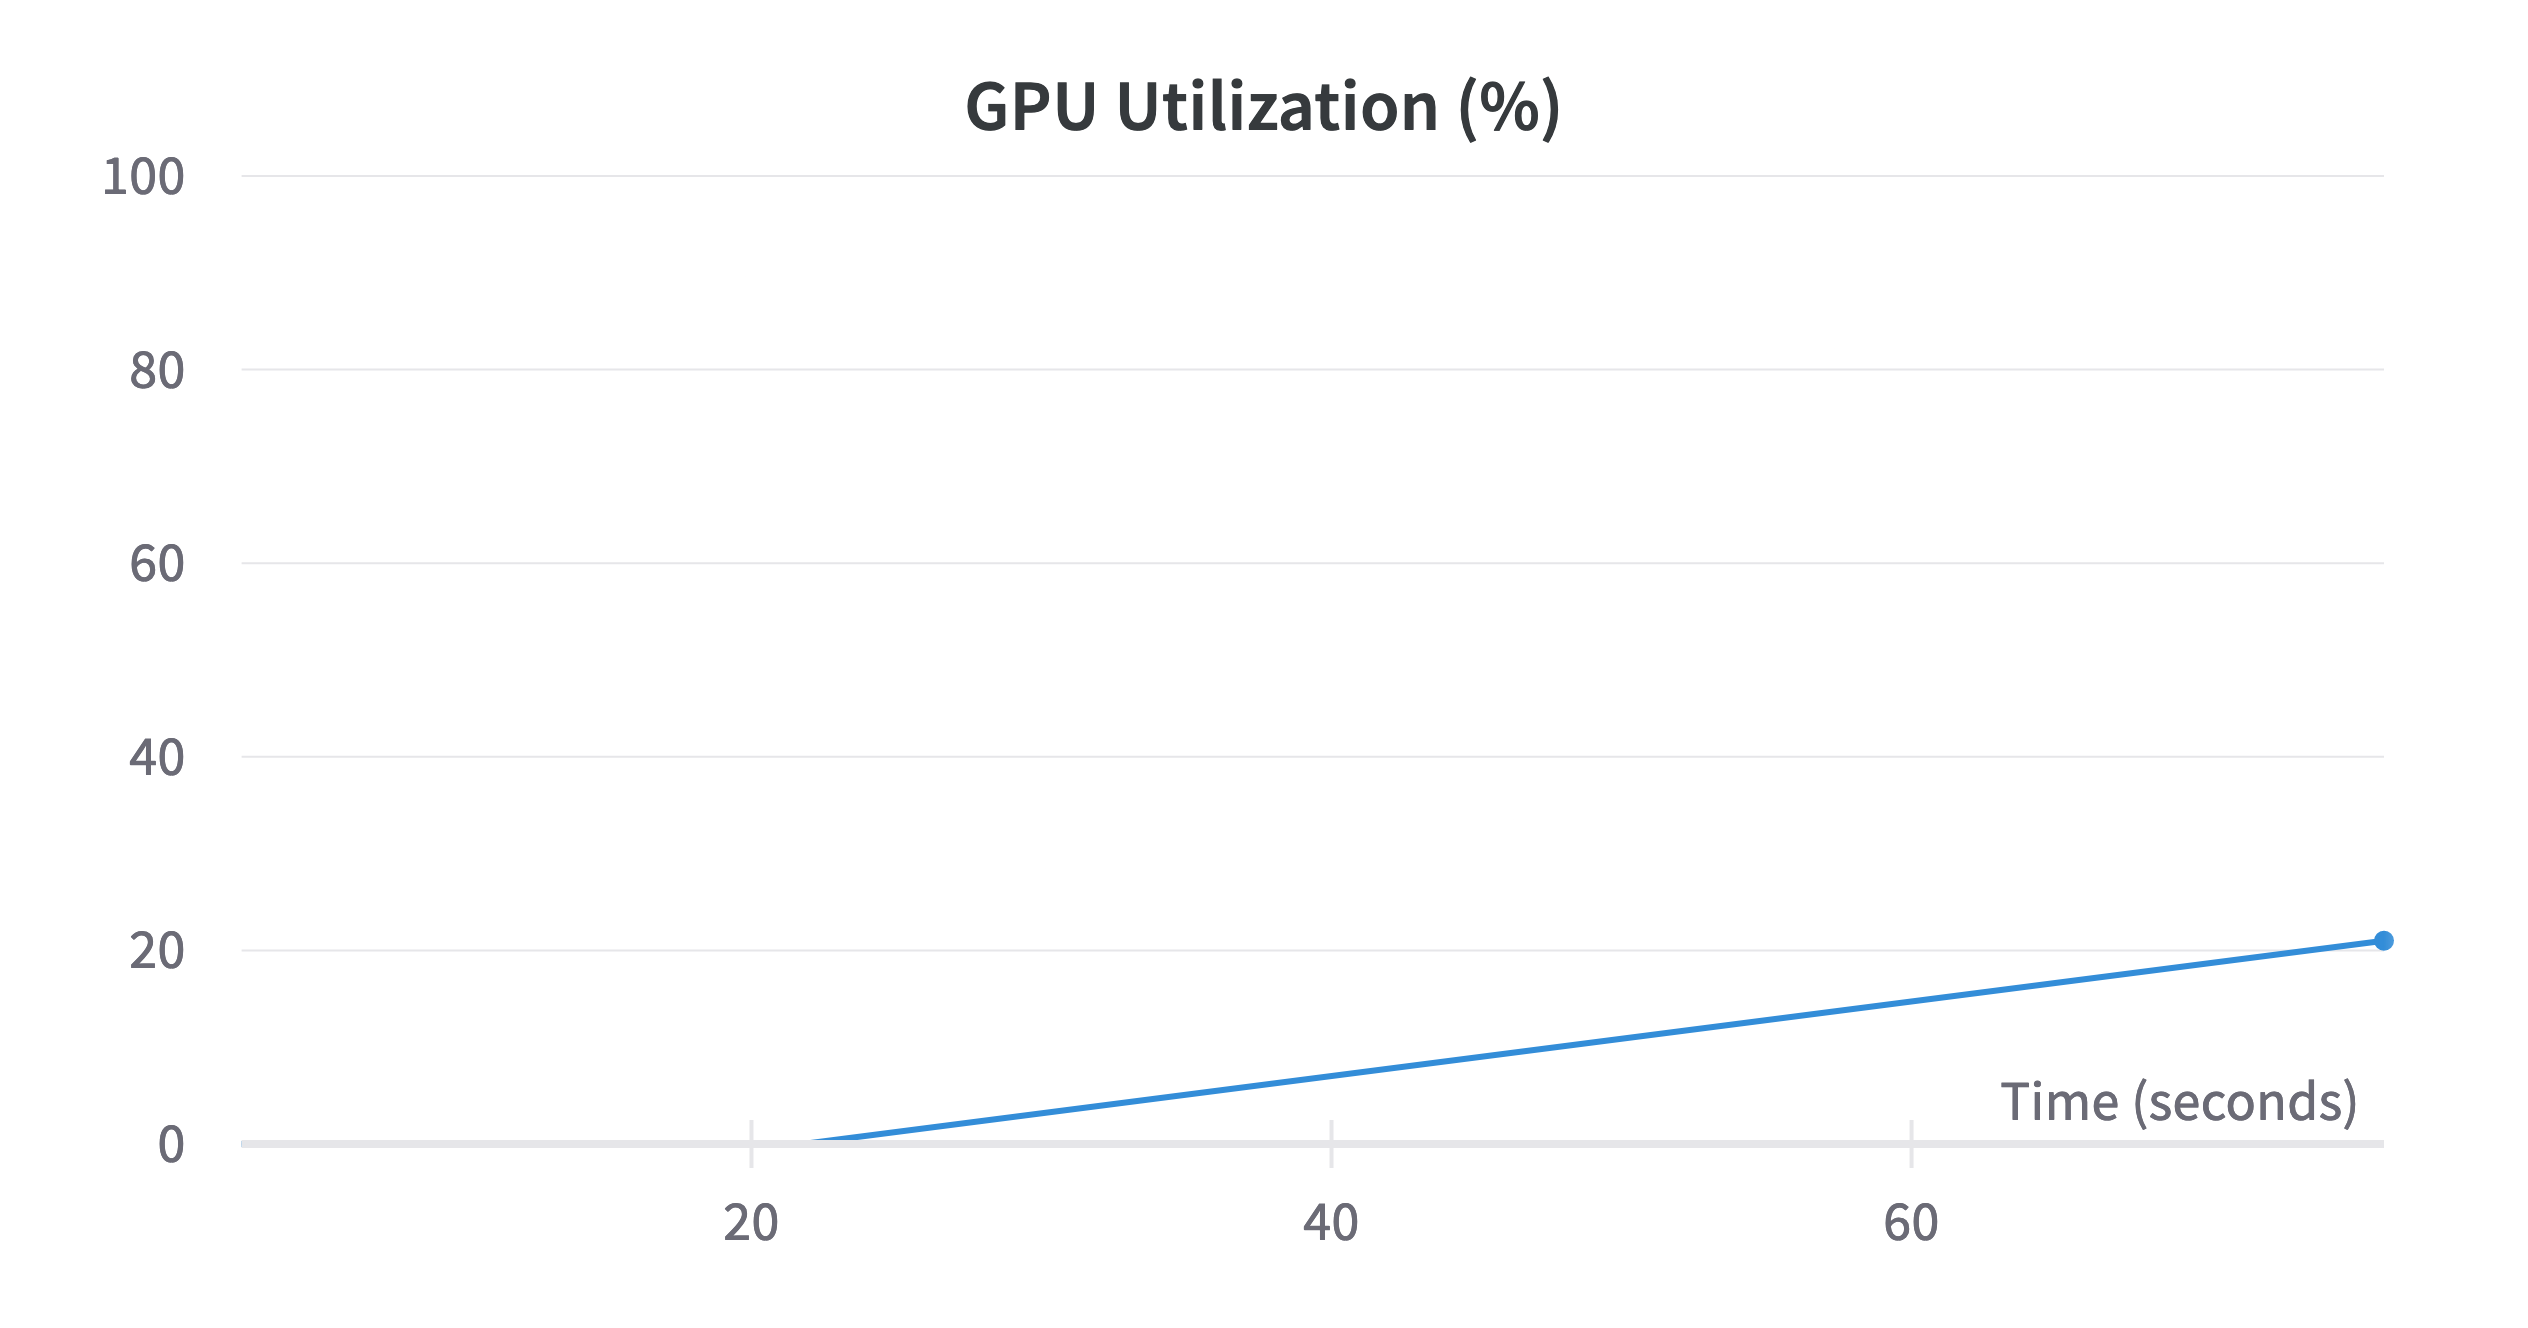
\includegraphics[width=\textwidth]{chapters/3_models/imgs/ufnc/ufcnusagevera.png}
	\end{subfigure}
	\hspace{.5cm}
	\begin{subfigure}{0.43\textwidth}
		\centering
		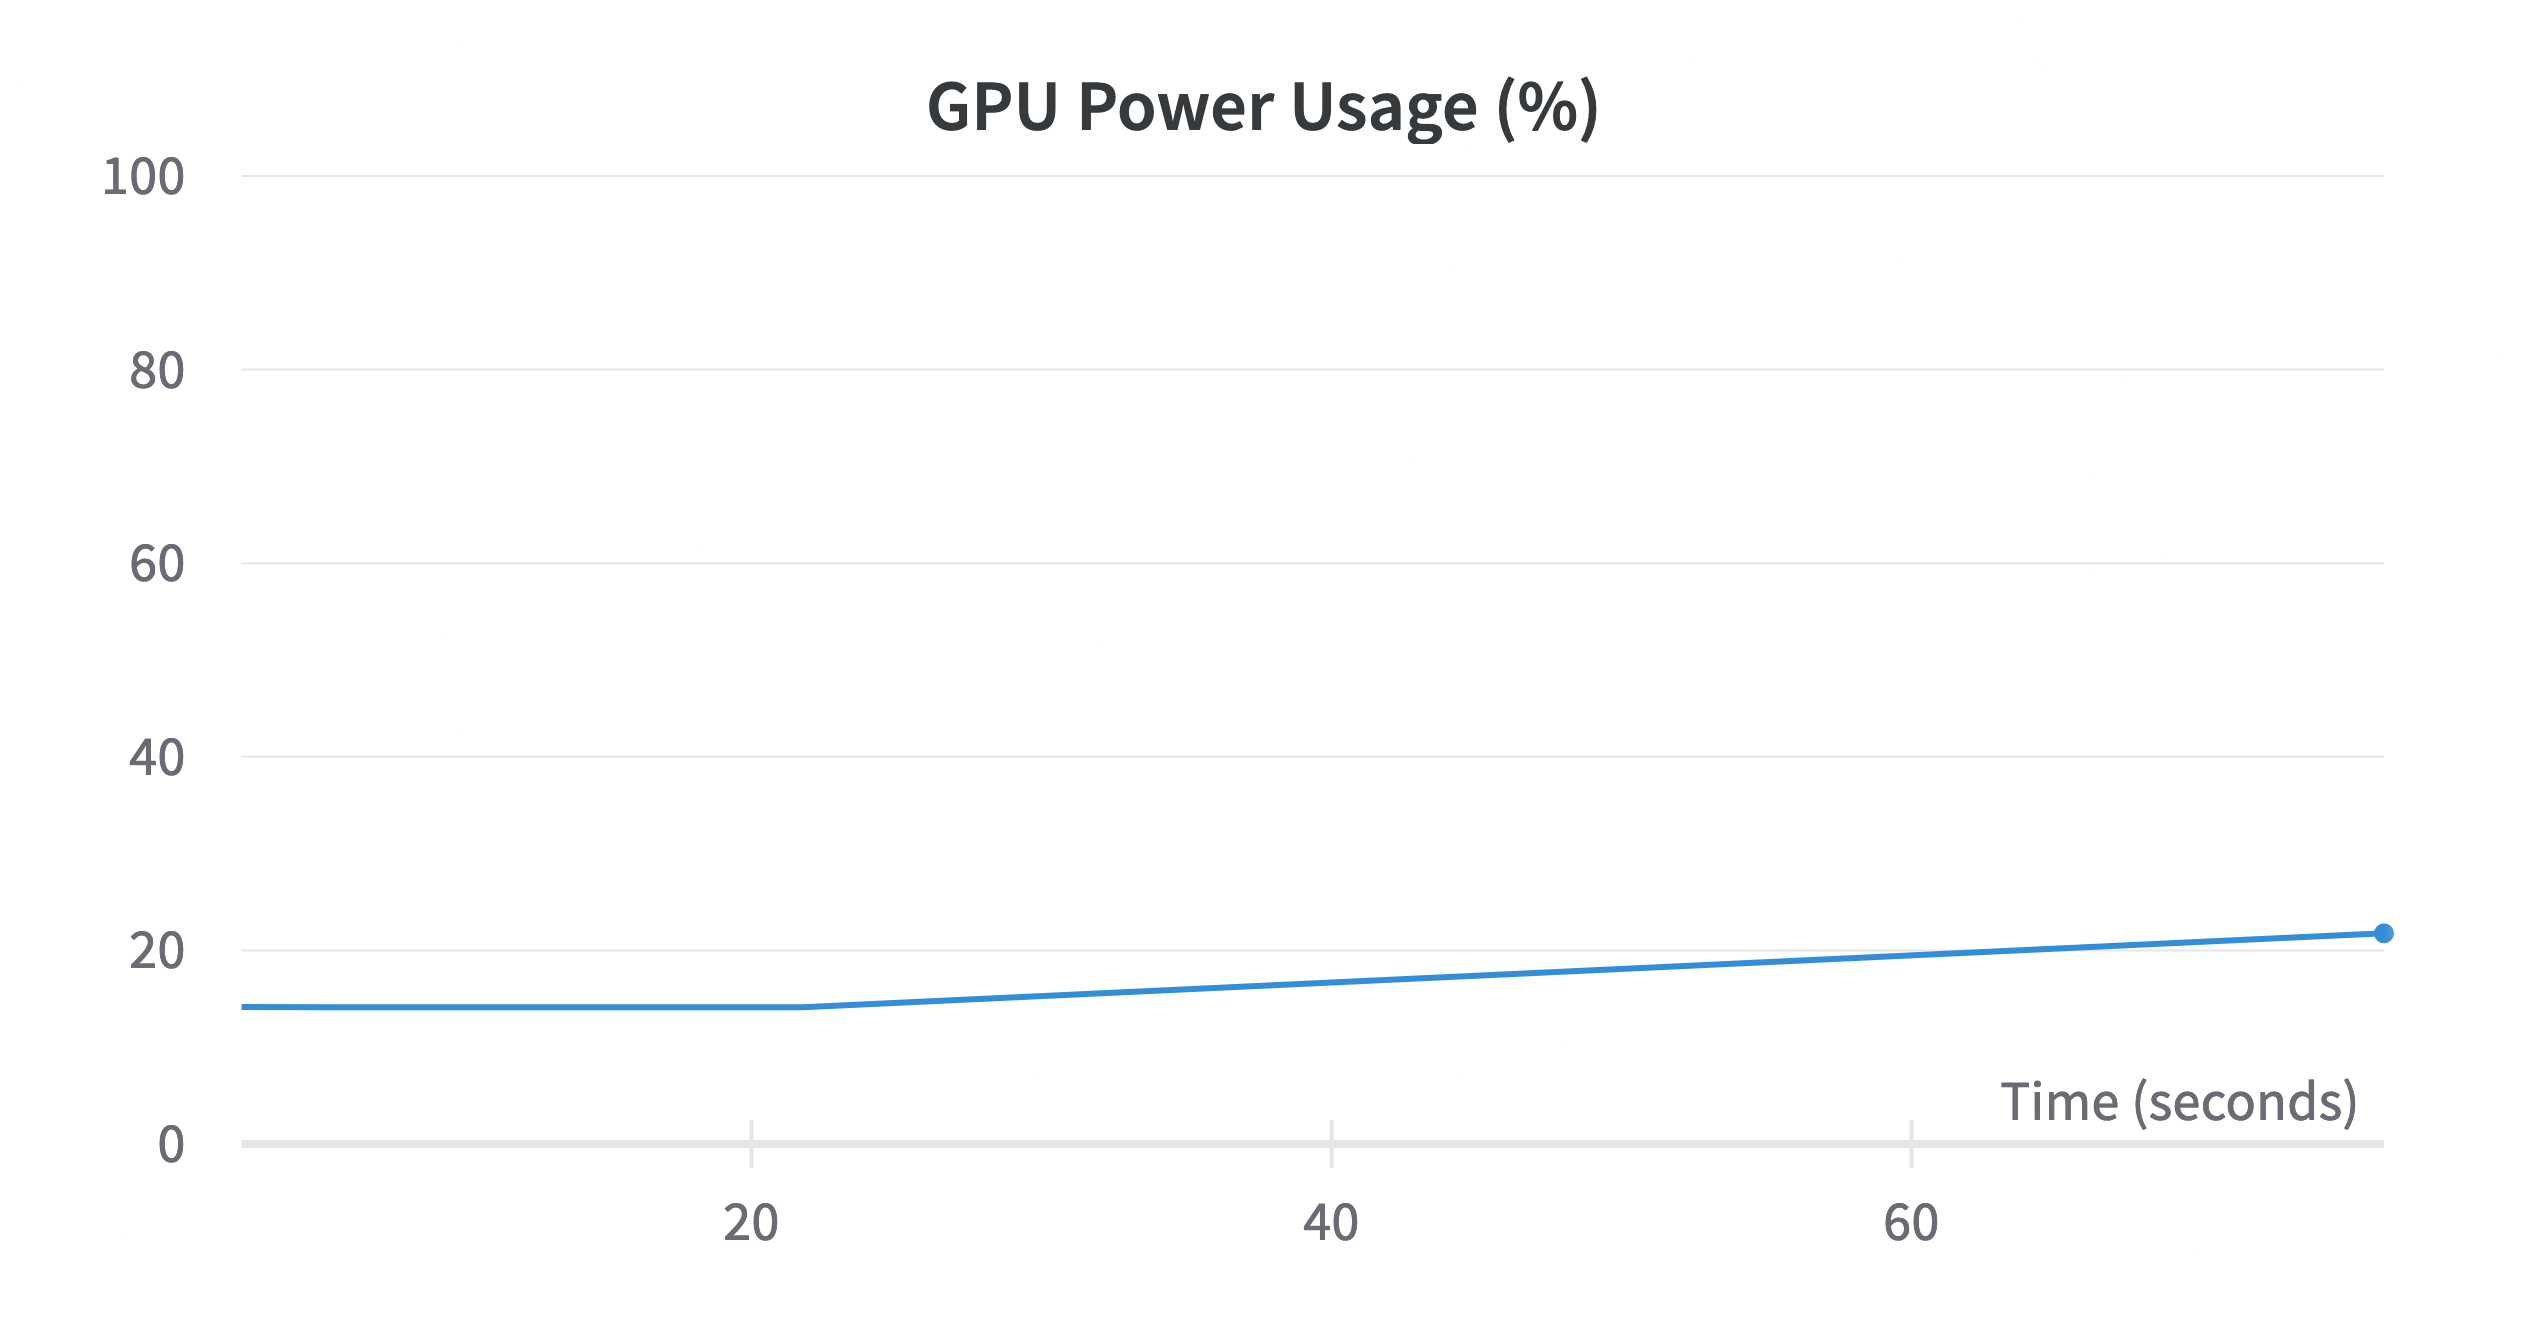
\includegraphics[width=\textwidth]{chapters/3_models/imgs/ufnc/ufncusageperc.png}
	\end{subfigure}\\
	\begin{subfigure}{0.43\textwidth}
		\centering
		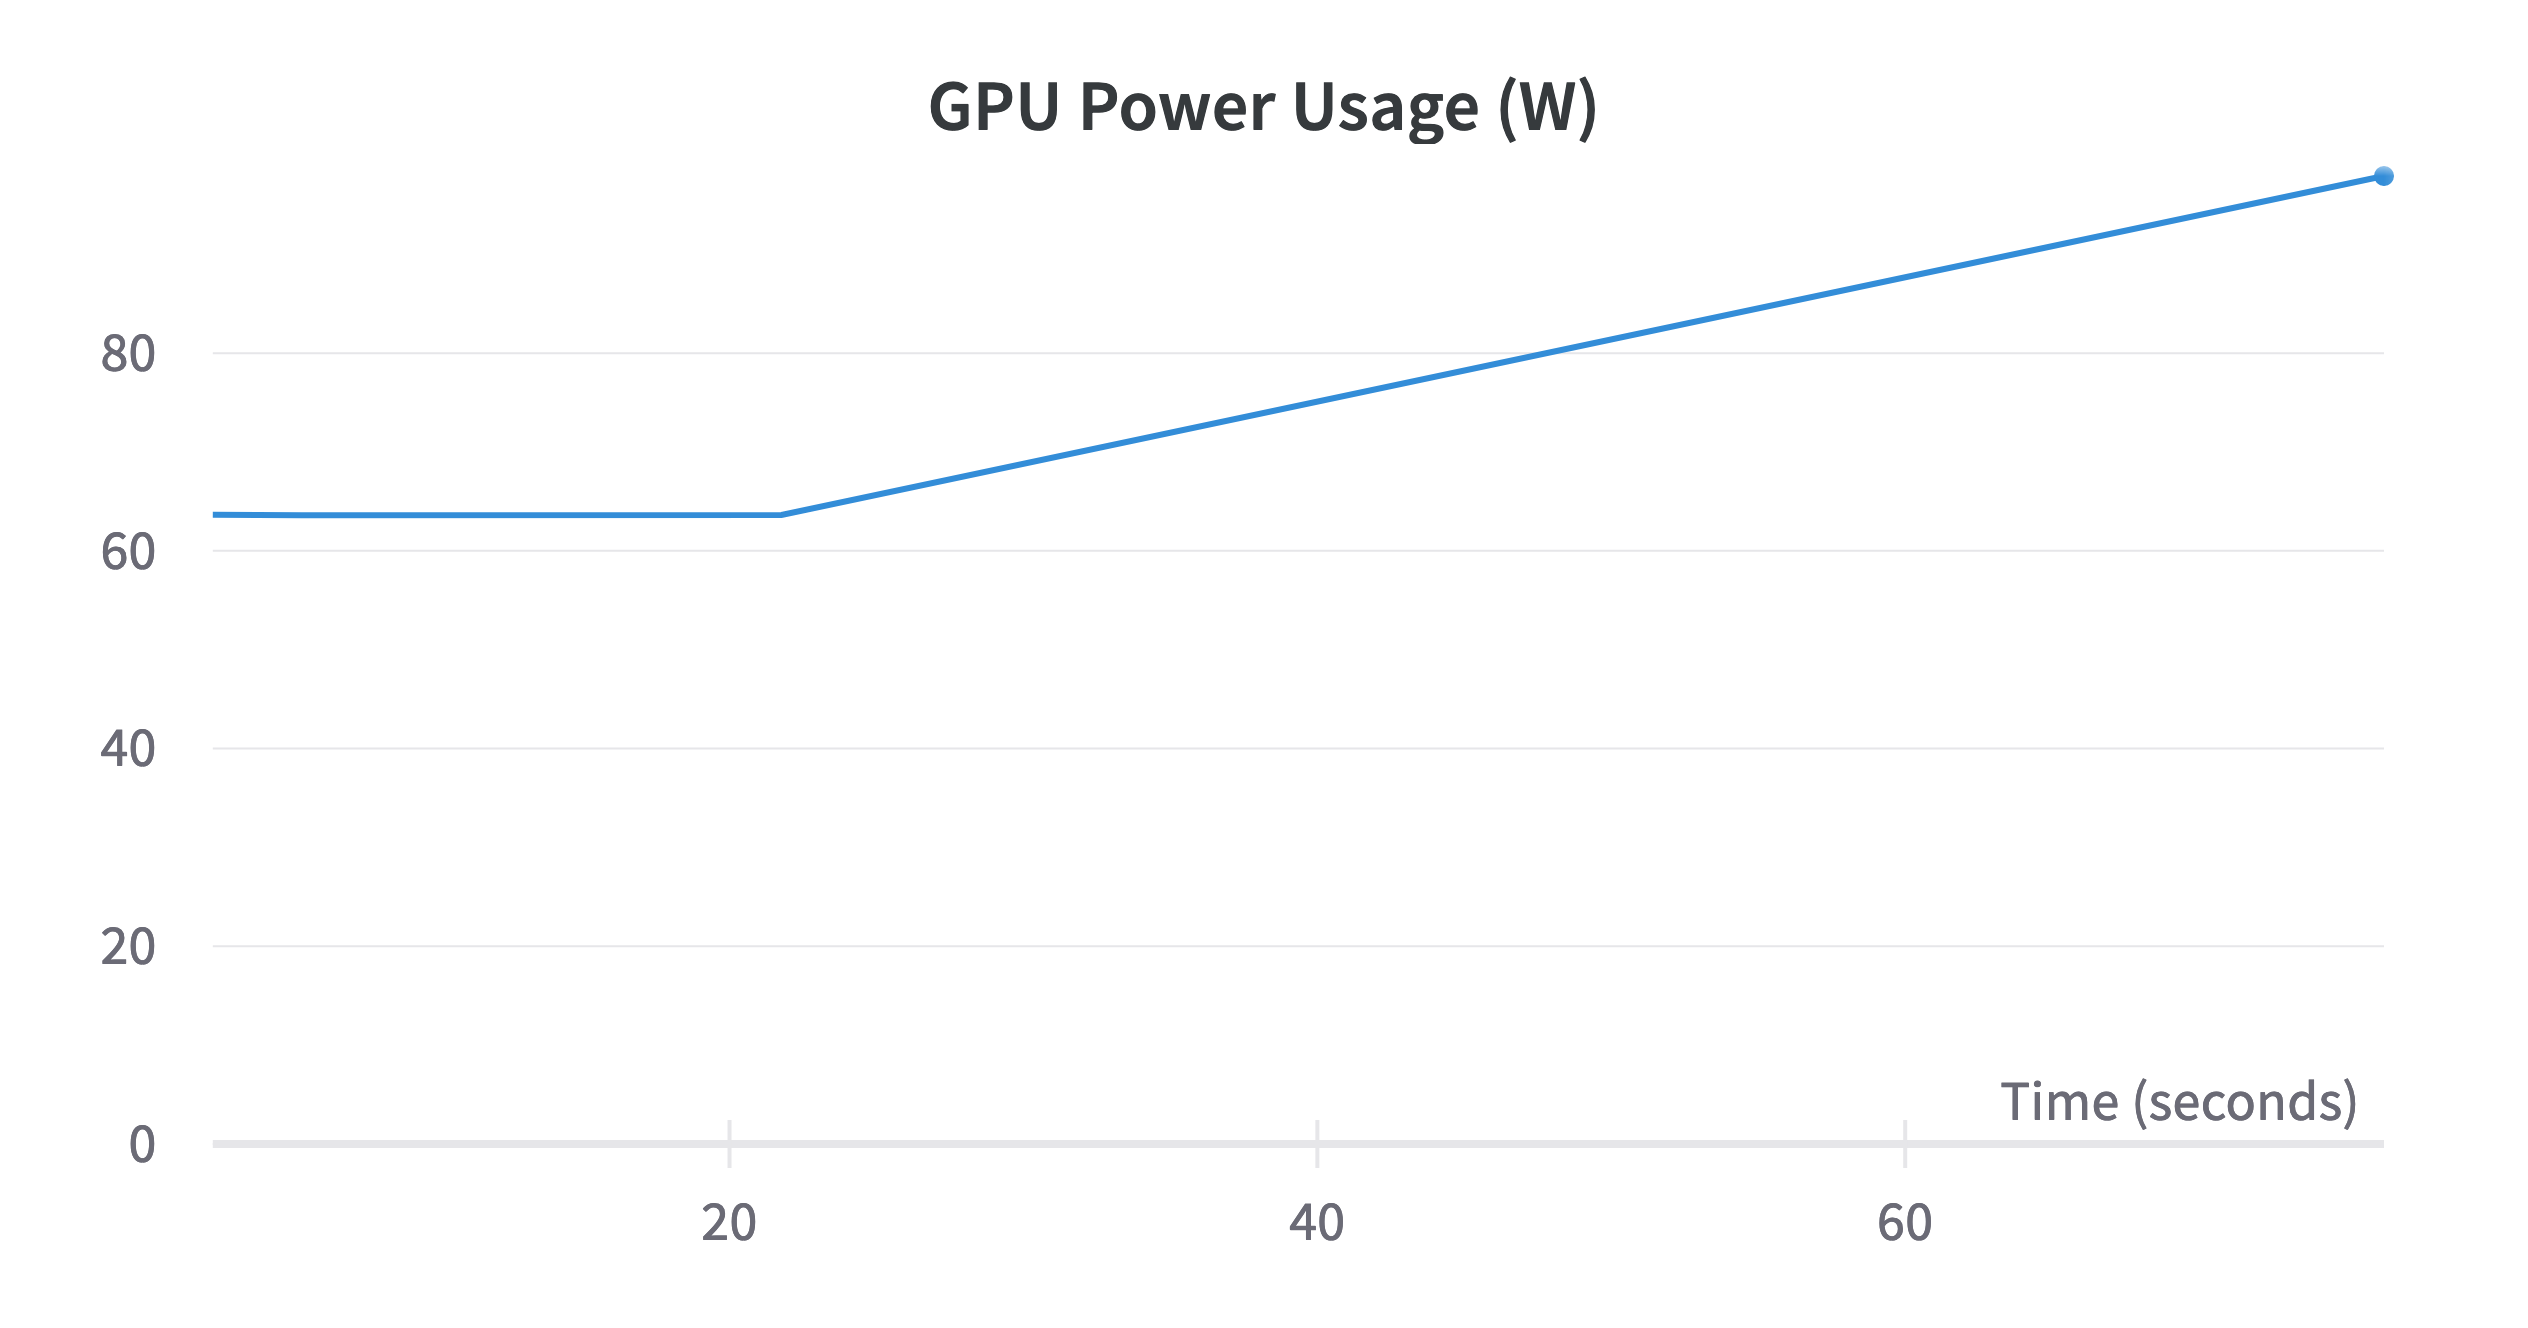
\includegraphics[width=\textwidth]{chapters/3_models/imgs/ufnc/ufncusagew.png}
	\end{subfigure}
	\hspace{.5cm}
	\begin{subfigure}{0.43\textwidth}
		\centering
		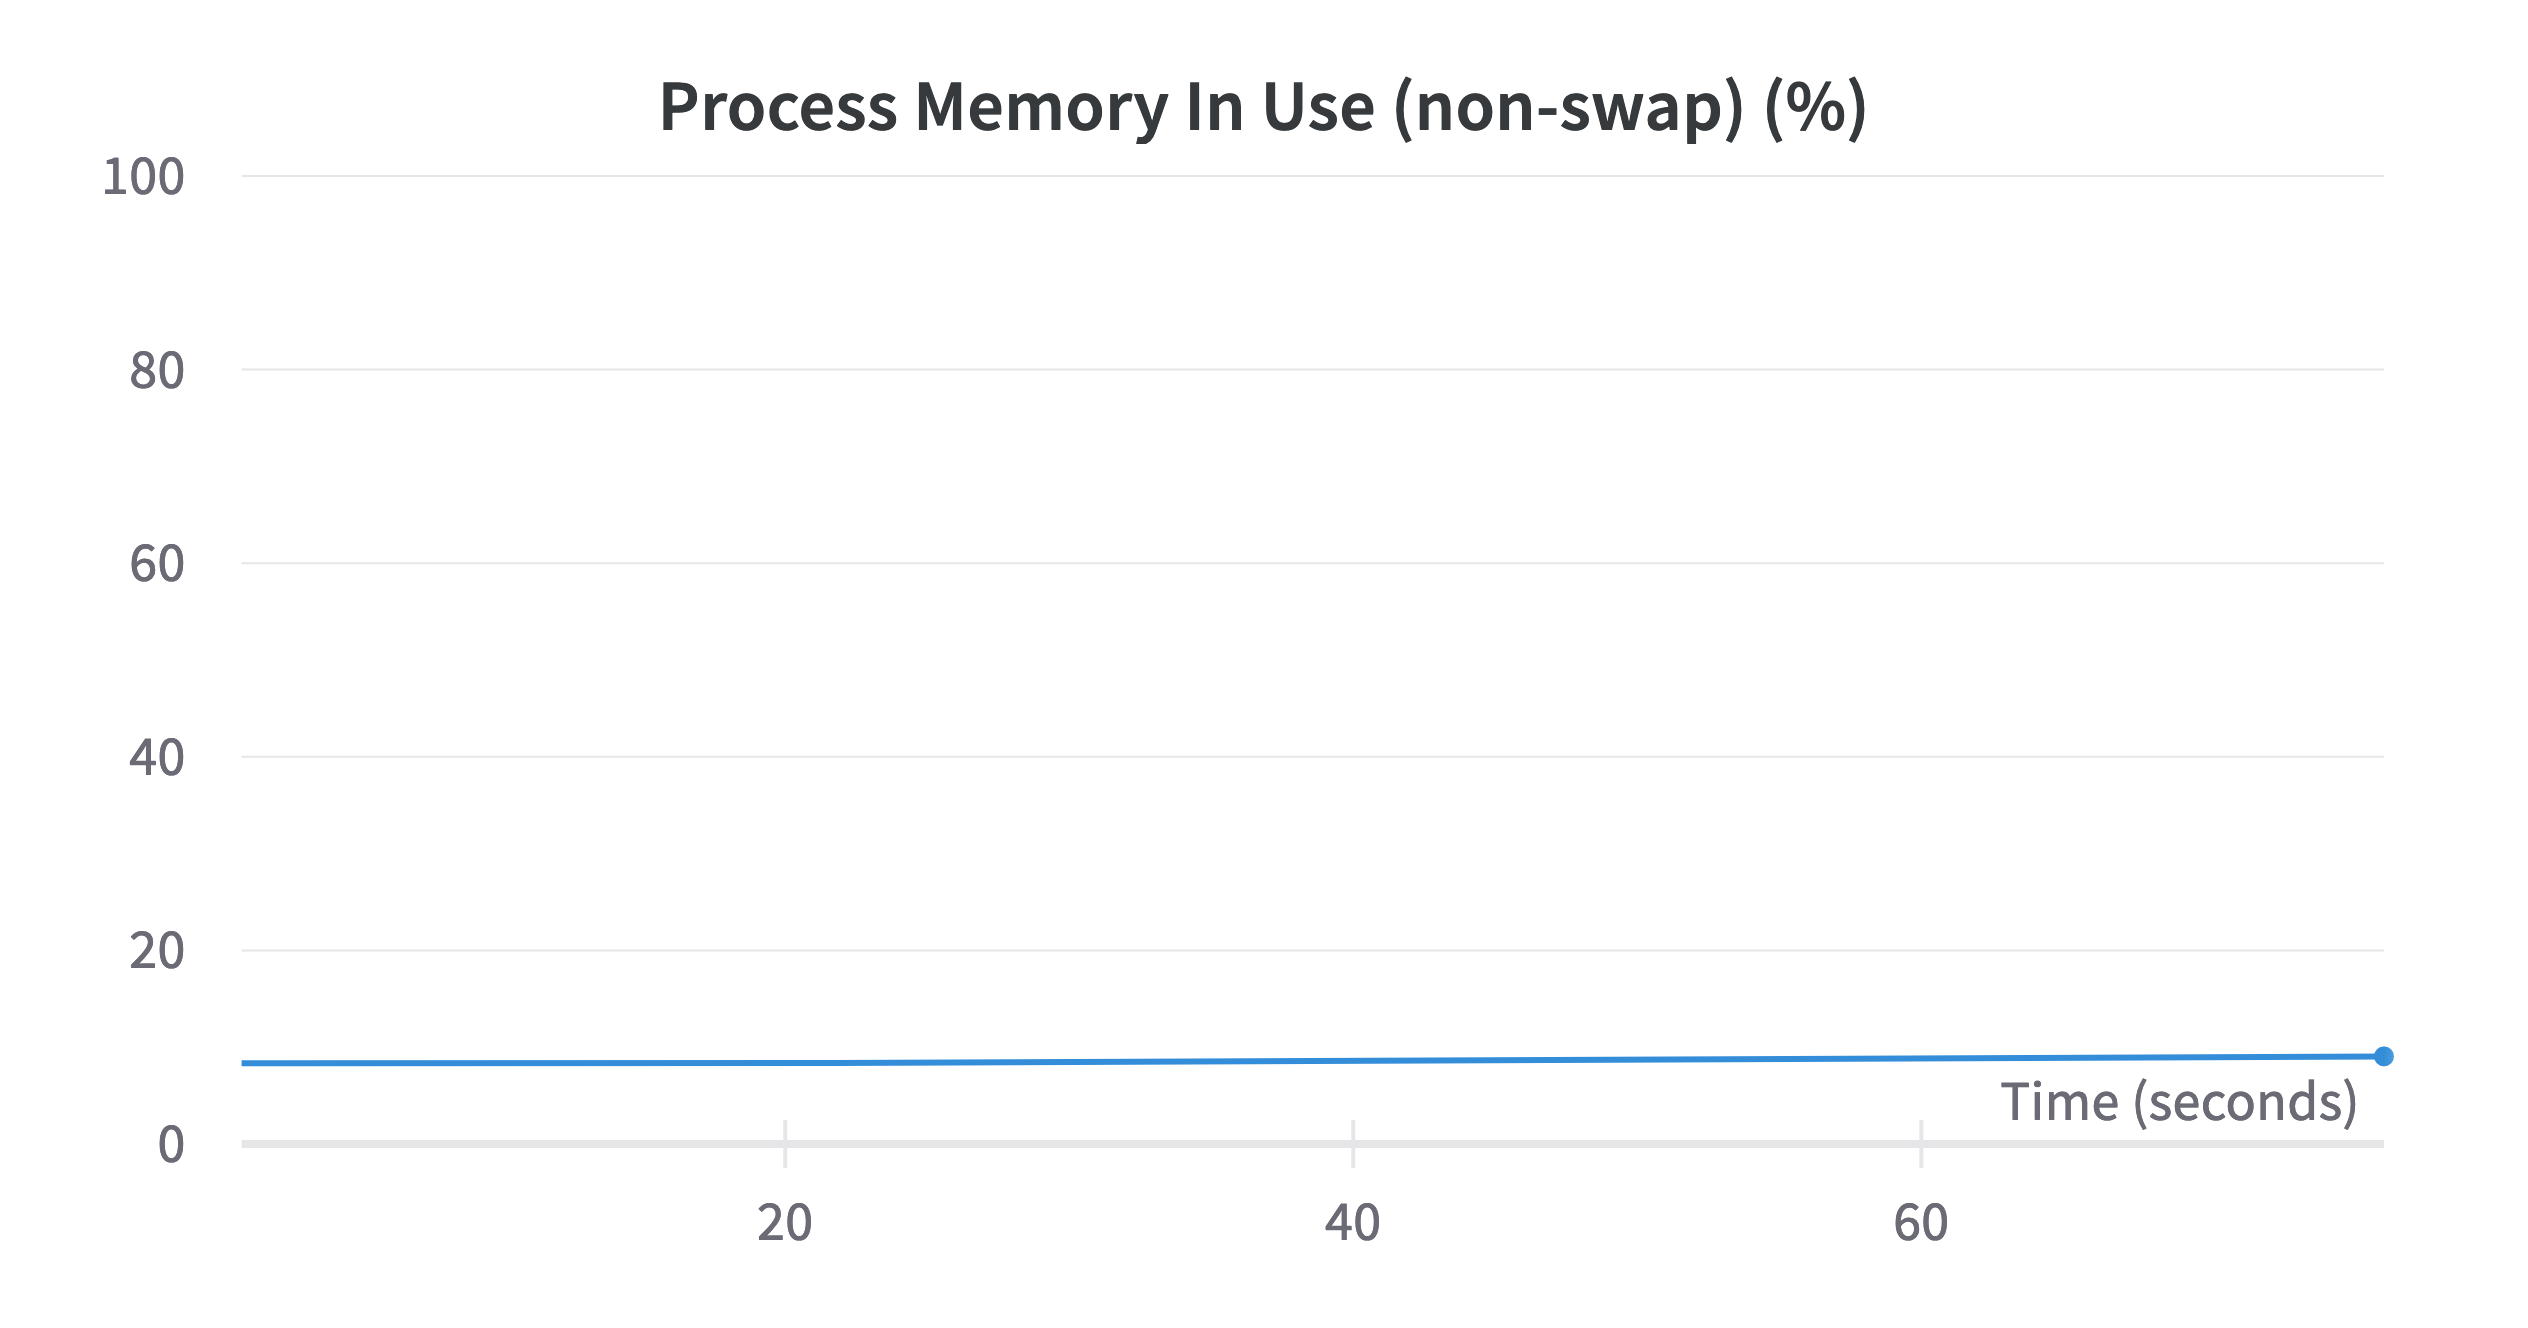
\includegraphics[width=\textwidth]{chapters/3_models/imgs/ufnc/ufcnmemram.png}
	\end{subfigure}\\
	\caption{System resources utilized during the Training phase.}
	\label{fig:ufcnsysusage}
\end{figure}

\begin{algorithm}[H]
	\caption{MLP model Training Algorithm}\label{alg:ufcntraining}
	\begin{algorithmic}
		\Require train/validation datasets; Baseline Neural Network Model

		\State Batch Size $\gets$ 10
		\State Learning Rate $\lambda \gets$ 0.01
		\State Epochs $\gets$ 100
		\State Patience $\gets$ 20
		\State loss $\gets$ L1Loss()
		\State Optimizer $\gets$ Adam Optimizer
		\State
		\For{\textbf{each} epoch \textbf{in} epochs}
		\For{\textbf{each} (batch\_id, before, after, target) \textbf{in} train.next\_batch()}

		\State train\_prediction $\gets$ model(before, after) \Comment{Model inference}
		\State train\_prediction $\gets \frac{\text{train\_prediction} \cdot \sum\text{train\_prediction}}{\sum target}$ \Comment{Area normalization}
		\State train\_loss $\gets$ loss(train\_prediction, target)
		\State Optimizer step
		\State Back Propagation
		\EndFor
		\State stop computing gradient
		\For{\textbf{each} (batch\_id, vbefore, vafter, vtarget) \textbf{in} validation.next\_batch()}
		\State val\_prediction $\gets$ model(vbefore, vafter) \Comment{Model inference}
		\State val\_prediction $\gets \frac{\text{val\_prediction} \cdot \sum\text{val\_prediction}}{\sum vtarget}$ \Comment{Area normalization}
		\State val\_loss $\gets$ loss(val\_prediction, vtarget)
		\EndFor

		\State check for Early Stopping
		\State check for Save Best Result
		\State start computing gradient
		\EndFor
	\end{algorithmic}
\end{algorithm}

From the training phase graph shown in Figure~\ref{fig:ufcntraining},
we can see that it has concluded successfully because the two curves
(training loss and validation loss) do not diverge but remain at a
relatively constant distance from each other.
This also suggests that there is no overfitting.
However, the values of the two loss functions do not appear to decrease
significantly as the epochs progress, indicating that the model may
not have generalized well.

From the graphs in Figure~\ref{fig:ufcnsysusage}, it is apparent that the
machine on which this model was trained was relatively underutilized.
In particular, it's worth noting that GPU utilization did not exceed 30\%,
and GPU memory was barely utilized, staying at around 20\%.
This suggests that the model can be trained on less powerful machines as well.
The model is also relatively lightweight in terms of memory,
with just 100 MB (see Table~\ref{tab:ufcnspecs}), and the training time
did not exceed 30 seconds.
Inference time is extremely fast, taking less than a second.

